\documentclass[12pt]{article}
\usepackage{graphicx}
\usepackage{lscape}
\usepackage{natbib}
\usepackage[top=1in, bottom=1in, right=1in, left=1in]{geometry}
\usepackage{setspace}
\usepackage[reqno]{amsmath}
\usepackage{mathtools}
\usepackage{amssymb}
\usepackage[hidelinks]{hyperref}
\usepackage{subfig}
\usepackage{bibentry}
\usepackage{array}
\usepackage{dcolumn}
\usepackage{url}
\usepackage{makecell}
\usepackage{float}
\DeclareMathOperator{\ExpOp}{E}
\DeclarePairedDelimiterX{\ExpArg}[1]{[}{]}{#1}
\newcommand{\E}{\ExpOp\ExpArg*}

\begin{document}

\title{Homework 1 \\
        \large PLSC 597}

\author{Taran Samarth}
\date{\today}
\maketitle

\onehalfspacing

\section*{Problem 1}

\subsection*{Part 1}

$\hat{\rho}$ is unbiased for $\rho$ if $\E{\hat{\rho}} = \rho$.

\begin{align*}
\E{\hat{\rho}} & = \E{\E{\hat{\rho} | D_i}} && \text{(law of total exp.)} \\
& = \E{p(D_i = 0)\E{\hat{\rho} | D_i = 0} + p(D_i = 1)\E{\hat{\rho} | D_i = 1}} && \text{(def. of conditional exp.)}\\
& = \E{\frac{1}{2}\E{2Y_{1i}} + \frac{1}{2}\E{-2Y_{0i}}} && \text{(by linearity)} \\ 
& = \E{\E{Y_{1i}} - \E{Y_{0i}}} && \\
& = \E{Y_{1i} - Y_{0i}} = \rho &&
\end{align*}

The statement is true.

\subsection*{Part 2}

In class, it was said that $\hat{\rho}$ is a consistent estimator of $\rho$ as $N \rightarrow \inf$. For a fixed $i$ and $D_i$, the population has no effect on the estimator (the outcome of the single unit does not depend on the size of the population--only on the treatment assignment in the switching equation). (My intuition prior to class was that this is inconsistent because the value should switch, depending on the treatment assignment, between $2Y_{1i}$ and $-2Y_{0i}$, so the estimator does not necessarily converge to a single value. Convergence is necessary for consistency.)

\section*{Problem 2}

\begin{table}[H]
\begin{tabular}{p{1in}|p{1in}|p{1.5in}|p{3in}}
Article & Causal effects & ID strategies & Ideal intervention and manipulability\\
\hline
\citet{Miller2023} & ATE of Congressmember gender on being interrupted in hearings & Implicitly estimating the difference in the average likelihood of being interrupted for Congresswomen, compared to Congressmen & Running hearings with randomly-assigned Congresspeople, witnesses, seating arrangements, chairs, and topics, and estimating the average difference in the number of interruptions between Congressmen and Congresswomen. This generally seems manipulable, since the committee room, rules for speaking, etc. could be standardized for each hearing.\\
\hline
\citet{Naurin2023} & ATE of being in different stages of pregnancy and parenthood on political engagement (seemingly among heterosexual couples) & Estimating difference in avg. levels of political engagement between treated (pregnant/parent) and control (matched over gender, age, education, and interview time) groups & Randomly assigning half of a sample of heterosexual couples to bear children (and the rest to not) and measuring their levels of political engagement over 9 months or more. Such an experiment would effectively manipulate the cause, assuming the groups are balanced on covariates like socioeconomics, but the estimated effect is going to capture a lot of other information (e.g. couples might be more likely to split without a child, so the ATE on political engagement may account for parenthood and its other downstream effects---not parenthood in isolation).
\end{tabular}
\end{table}

\section*{Problem 3}

\subsection*{Part 1}

As visualized in Figure \ref{fig:hists}, $X$ is not strongly skewed (has a mild right tail) and is roughly symmetric. $Y$ is strongly right-skewed and is not symmetric.

\begin{figure}[H]
\caption{X and Y Histograms}
\label{fig:hists}
\centering
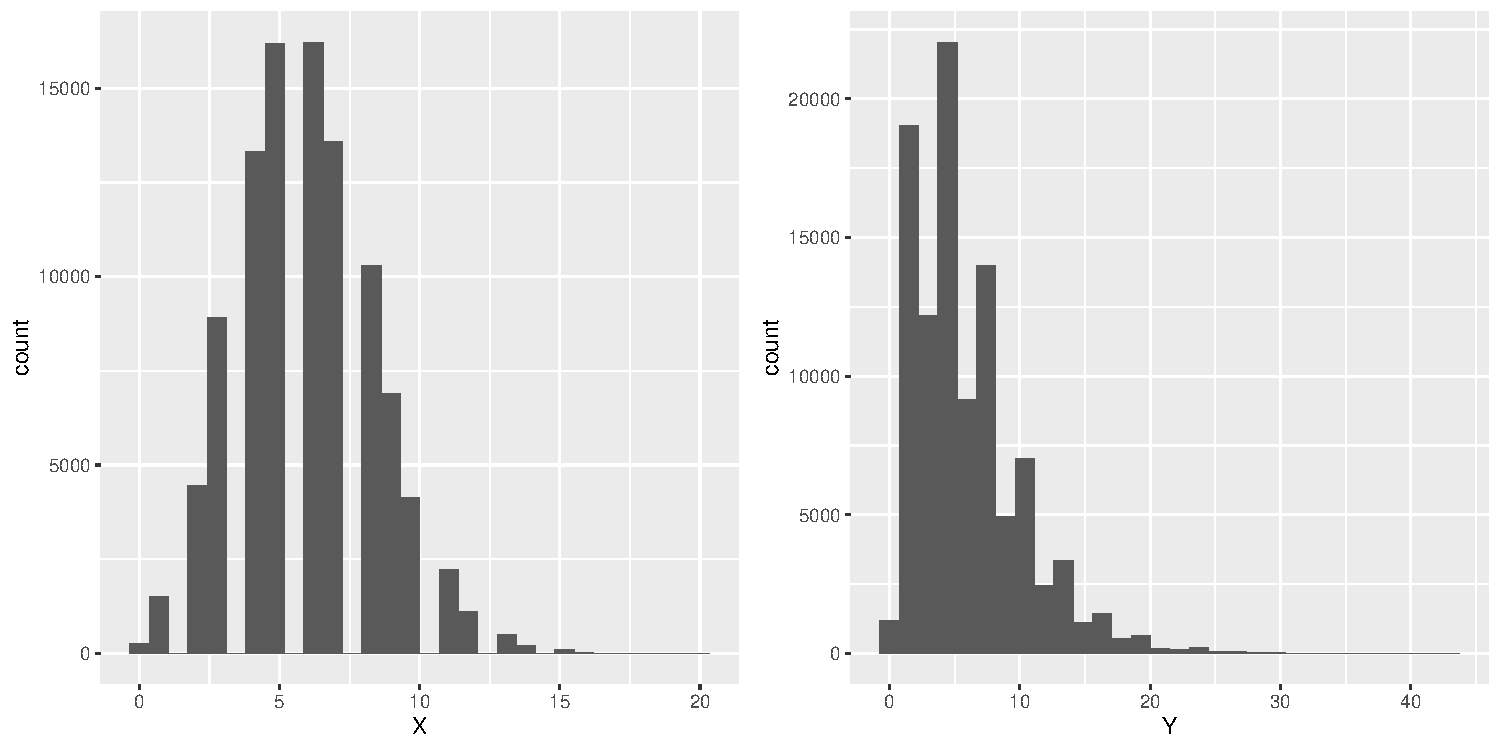
\includegraphics[width = .8\textwidth]{hw1_hists.pdf}
\end{figure}

\subsection*{Part 2}

As shown in Figure \ref{fig:x_hists}, the distribution of the mean of $X$ converges to normality pretty quickly (unsurprising since the distribution of $X$ is close to normal), while, as shown in Figure \ref{fig:y_hists}, the distribution of the mean of $Y$ converges clearly to normality with sample size of 100 and greater (which is unsurprising since the distribution of $Y$ is not normal).

\begin{figure}[H]
\caption{X Histograms}
\label{fig:x_hists}
\centering
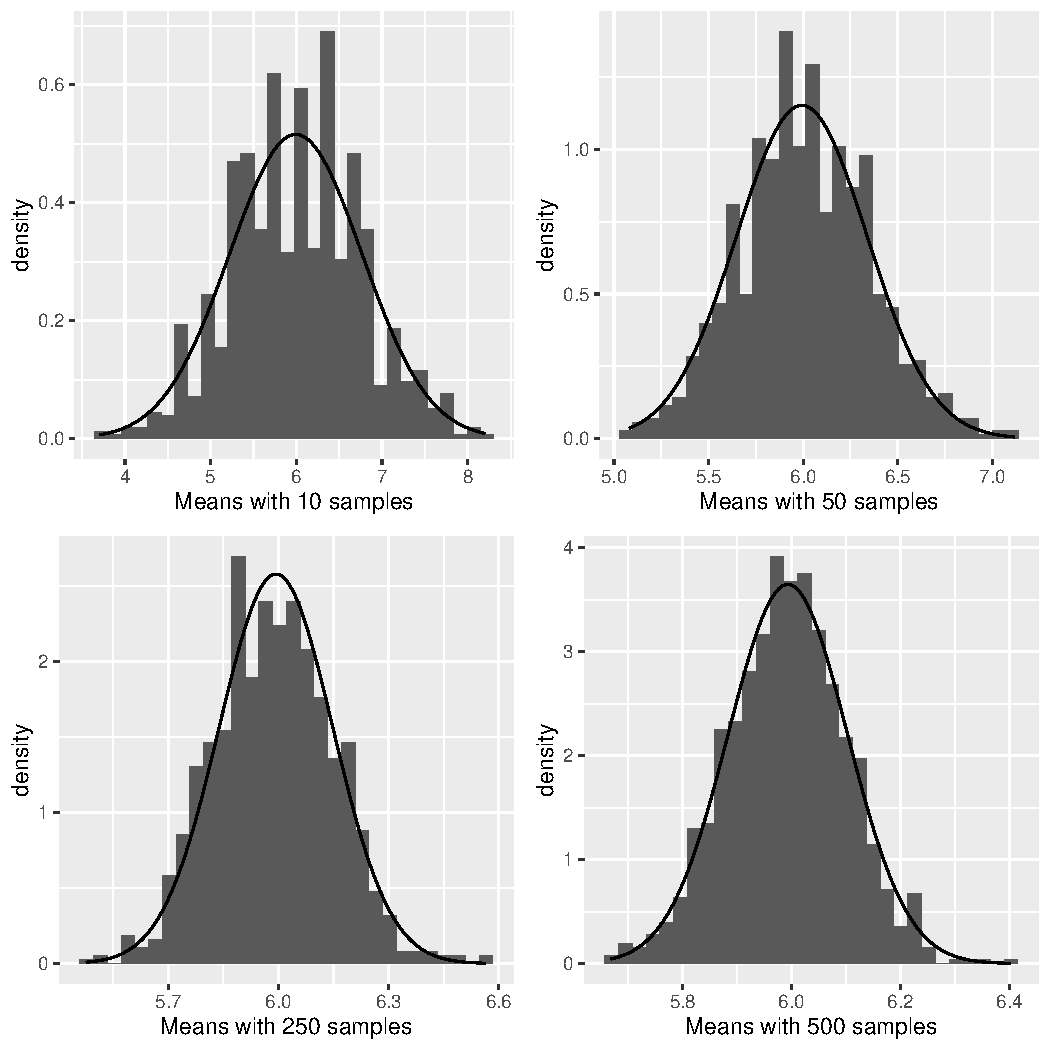
\includegraphics[width = .7\textwidth]{hw1_Xconv.pdf}
\end{figure}

\begin{figure}[H]
\caption{Y Histograms}
\label{fig:y_hists}
\centering
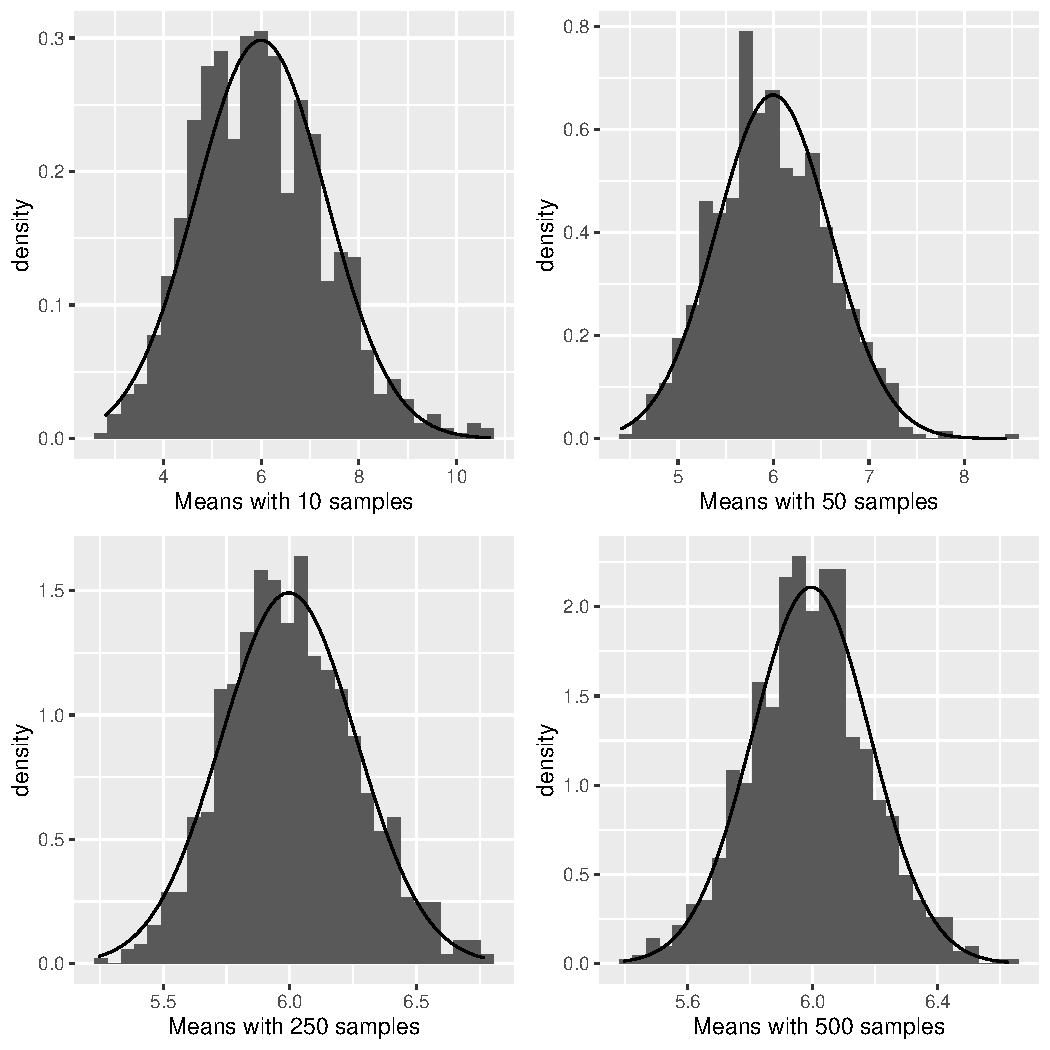
\includegraphics[width = .7\textwidth]{hw1_Yconv.pdf}
\end{figure}

\subsection*{Part 3}

The difference of means ($\bar{X} - \bar{Y}$) seems to converge rather quickly to normality: there's a slight left tail with 10 and 50 samples, but the distribution is more symmetric and normal with 100 or more samples.

\begin{figure}[H]
\caption{Diff. of Means Histograms}
\label{fig:diff}
\centering
\includegraphics[width = .7\textwidth]{hw1_diffmeans.pdf}
\end{figure}


\bibliographystyle{apsr}
\bibliography{hw1.bib}


\end{document}
